\documentclass[a4paper,12pt]{article}
\usepackage[utf8]{inputenc}

%paquetes
\usepackage{graphicx}
%\usepackage[spanish]{babel} 
\usepackage[spanish,es-tabla]{babel}
\usepackage[utf8]{inputenc}
\usepackage[document]{ragged2e}
\usepackage{amsmath}
\usepackage{textcomp}
\usepackage{float}
%\usepackage{subfig}
\usepackage{multirow}
\usepackage{multicol}
\usepackage{amsmath}
\usepackage[utf8]{inputenc} 
\usepackage{multirow} 
\usepackage{graphicx} % figuras
\usepackage{subfigure} % subfiguras
%\usepackage{subcaption}

\usepackage[dvipsnames]{xcolor}
\usepackage[footnotesize]{caption} %pone el texto de las figuras mas chico
%\use{multirow}
\usepackage{graphicx}
\usepackage{subcaption}
\newcommand{\grad}{$^{\circ}$}

%caracteristicas de paginas
\pdfpagewidth 8.5in
\pdfpageheight 11in
\setlength\oddsidemargin{-0,21in}
\setlength\evensidemargin{-0,21in}
\setlength\topmargin{-2cm}
\setlength\textwidth{7in}
\setlength\textheight{23.7cm}
\setlength\parskip{0.1in}
\title{Cuaderno Digital}
\usepackage{natbib}
\usepackage{graphicx}

\begin{document}

\maketitle
\section{14-05}
\subsection{Notas de Clase}
Al informe se le pueden agregar cosas
\subsubsection{Concurrencia y paralelismo}
Nociones basicas para la construccion de un soft

Maquina de Turing y maquina moderna opera sobre las mimas ideas opera sobre memoria y se transforma en una instrucción 
Hard y Soft leen instru y operan sobre ellas 
En las compus necesito una interrupción para interrupir el proceso (en las de turning esto no esta). 


Dedes el hard la interrupcion seria tocar una tecla (tambien se puede usar el soft) y el procesador tiene que dejar de hacer lo que esta haciendo y hacer otra. 

Una compu vieja con DOS no podia correr los dos programas juntos

En wind 3.11 se podian interruir los programas y pasarle la pelota a el otro. El sist operativo se encarga de las flechsa verdes y de gestionar que pasa con la memoria  !!
pero cada problema es responsable de interrupirse y se acuerda en donde quedó 

win 95: multitarea preventivo y le dice a un programa vos corta que necesito hacer otra cosa (no la tenia que hacer un programador)

single core: corre dos programas a la vez (PERO NO SIMULTANEO)
sistema multicore: cada uno corre uno

not concurrent not parallel una fila para una caja 
concurrent not parallel dos filas una vendedora 

parallel not concurrent dos cajas y cada fila va una boca (esto es mas rapido en bites (creo))
parallel y concurrent una sola fila para dos cajas (TIENE evento de coordinacion)

theard: un solo proceso puede tener distintos hilos corriendo en paralelo (no son simultaneos) (cada uno tiene una memoria) 

diferencia entre procesos e hilos :  los hilos tienen su propio espacio de almacenamiento temporal. Un proceso no comparten codigo y duplicar un proceso es mas pesado 

Con un solo proceso tengo que esperas que termine una tarea para empezar la otra. 
Para factorizar un numero: En cambio para multiproc puede empezar varias tareas a la vez 
porque lo hilos tardan mas que los procesos? Por los intercambios de info (porque cada uno tiene una memo interna)

En python: 3 librerias

multiprocessing  cpu bound

threading io bound

asyncio programa io bound sin threads

Recomendaciones: hacer un programa para un unico proceso y despues nos fijamos que cosa tenemos que paraleliza. 

\subsubsection{Objetivos de hoy}
diseñar experimeto que permita decidir que el osci y la placa mide en simultaneo o secuencia y ver cual es el tiempo


\section{Seguimos con las mediciones de la clase anterior}
Para el diodo dice german que con la compu no poodemos mandar una cuadradada y tenemos que usar un comparador y hace que si la señal es positiva la deja pasar. A la señal le tenemos que poner signo. 

El cable que anda en mi compu (rosa y verde), hay q usar el blanco y amarillo en la punta y rojo y negro en el cable.  

Lo que vamos a hacer es un circuito inversor con amplificacion de 1 a 10. Vamos a usar el programa de la otra vez. (EL DE GENERA TONOS). Con la compu enviamos una señal y la tomamos con el osci. Por otro lado esta misma señal para por el inversor y va para el osci. 
Con la compu queremos adquirir los datos de los dos canales del osci. 

EL OPA ES UA741.

Canal dos es la salida del circuito. 

\begin{figure}[H]
\centering
     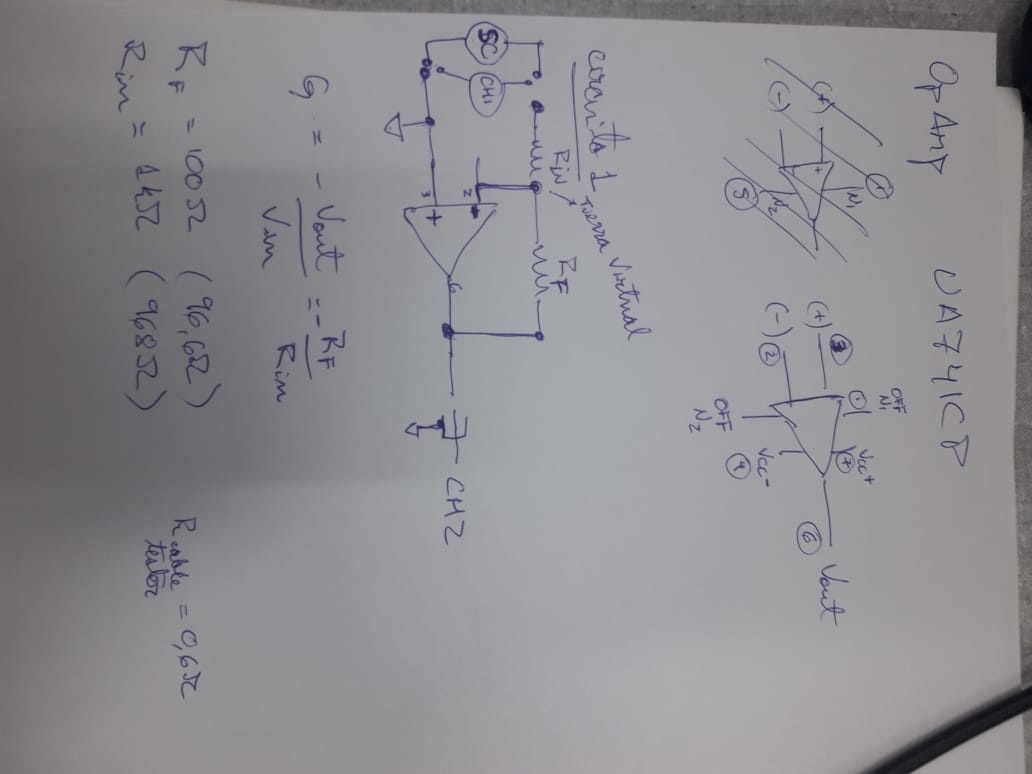
\includegraphics[scale=0.40]{NotasdelcirucitoyR.jpeg}
     \caption{Estan las patitas del ampli y las R que usamos y como es el circuito}
     \label{cir1}
\end{figure}

\section{Notas de clase}
Las placa de la compu funcionan indep del procesador. Buffer permite acumular datos.

Codigo en python ==> hilos y procesos 

import concurrent.futures
import  urllib.request

courrent.futures.ThradpoolExecutor creo una lista de tarea y las distribuye al hilo disponible. uso esta para cosas que me tengo que meter a internet  
Y tengo que garantizar la simultanidad de las cosas porque no todo lo puedo usar en hilos y eso
El acceso a la cola tiene que ser atomica 
se puede especificar la cantidad de hilos que puede usar 

executor.submit el primer parametro es funcion y despues toma los parametros de la funcion 


courrent.futures.as$\_$completed si se va completando tal accion que haga algo por ejemplo qe printee

El problema es io cound o cpu bound?
estructura de datos? 


\section{Seguimos con las mediciones del opamp}
El circuito no estaba invirtiendo. entonces El inversor no funciono porque no tenemos un punto fijo. La tierra de la alimentacion NO esta acoplada con todo lo otro. Entonces estabas alimentando al opamp con 0V. 

Damian nos dijo que podemos poner unas resistencias en +- in para mantener fijo el voltaje la diferencia de voltaje en 6Volt o hacer un circuito mas facil. Pasamos a un no inversor. Esto no tiene problemas porque no necesitamos que tenga un punto en comun.  Nos está dando 1.5 volt y le estamos mandando 1v. es raro 

\begin{figure}[H]
\centering
     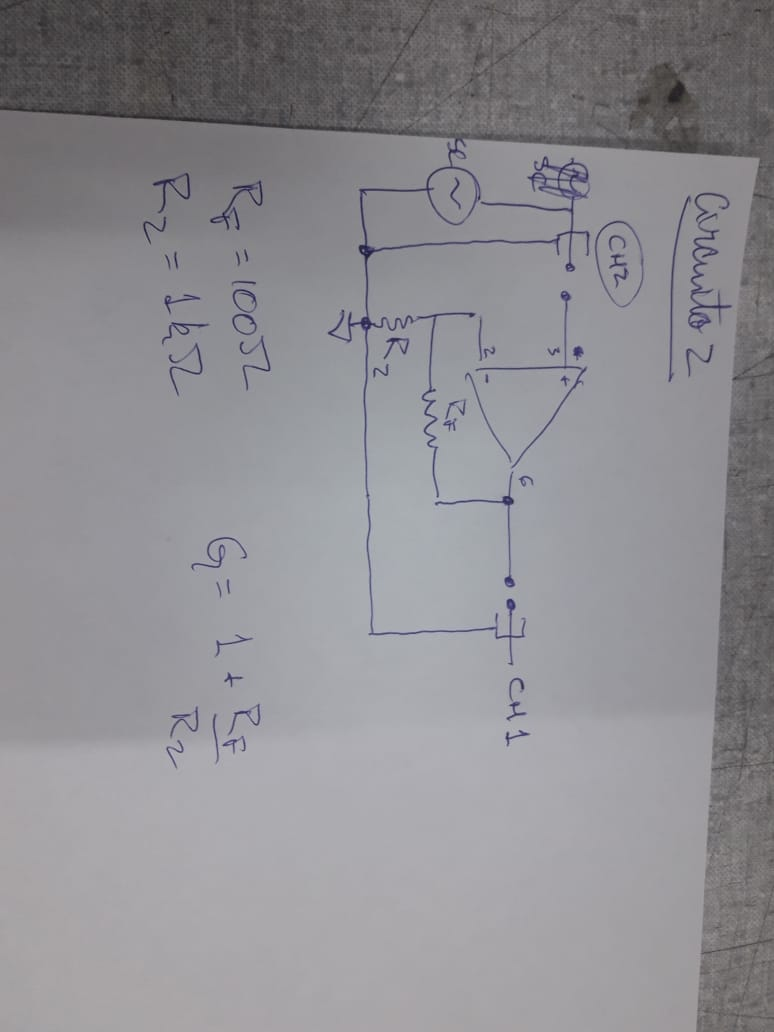
\includegraphics[scale=0.40]{CircuitoNoInversor.jpeg}
     \caption{circuito al que pasamos porque el otro no funciono. Estan las R}
     \label{cir2}
\end{figure}

Armamos uno todavia mas simple donde el voltaje de salida tiene que ser el mismo al de entrada. Un seguidor

Comentario de German: si entramos con una señal sino y el ampli de 0 y 10 v la parte negativa no entra al opam. Como se arregla? poniendo un div de tension. asi simepre entra 5. Y ponemos un cap para que solo pase alterna. 
y este pasa altos tendra un tiempo de corte que depende de C y r paralela. 

\begin{figure}[H]
\centering
     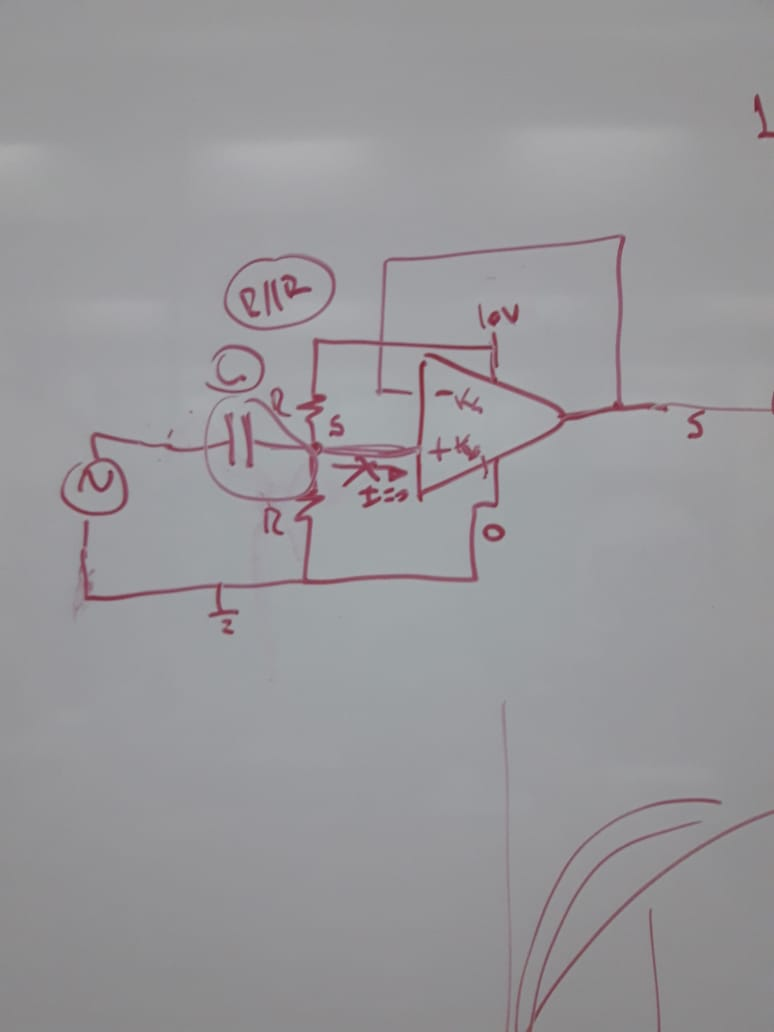
\includegraphics[scale=0.40]{comentariogerman.jpeg}
     \caption{circuito al que pasamos porque el otro no funciono. Estan las R}
     \label{cir}
\end{figure}

El ampli tiene una amplitud de minima de 1.3 o algo asi y como le dabamos con 1 no le metia. 

Armamos el div de tension: para poder entrar con la placa de la compu porque es ac. 
 
Manual del ampli:http://www.ti.com/lit/ds/symlink/ua741.pdf 


Finalmente este es el circuito que queremos y con el que mañana medimos 

\begin{figure}[H]
\centering
     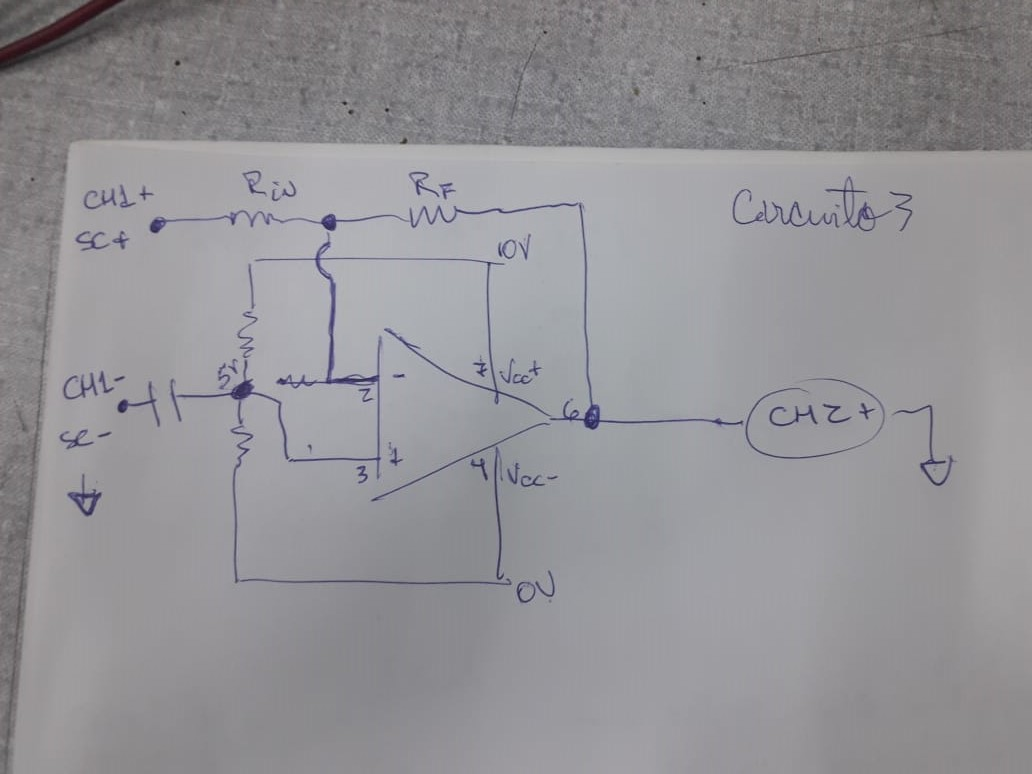
\includegraphics[scale=0.40]{Circuitofinal.jpeg}
     \caption{circuito Final que usamos}
     \label{cir_final}
\end{figure}

\section{Dia 15/05}

Hoy la idea es hacer un barrido de frec para el opamp y si llegamos hacemos de ver el tiempo de subida/bajada en el opamp. 

OBS: el generador tiene que estar en high z

La señales que enviamos con la compu es de 1V y el volumen está al maximo. 


Primero tomamos para ganancia 0.1. 
R in era de 1000 Ohm
Rf 100Ohm


Paso algo re raro: la ganancia 1 no nos funciono porque estaba monton en 9.2 v y no funcionaba porque la salida del opamp da hasta masomenos 8.5 v

Entonces damian nos dijo que referimos la salida de la compu a un voltaje fijo (creo que 5 o algo asi).   con dos resistencia de 10k y no afecta nada. También, hay un capacitor en la entrada en serie para sacar la conti de la plca (el otrocap el de ayer es para subir y que no haya negativa). Ver figura \ref{comentario damian}


\begin{figure}[H]
\centering
     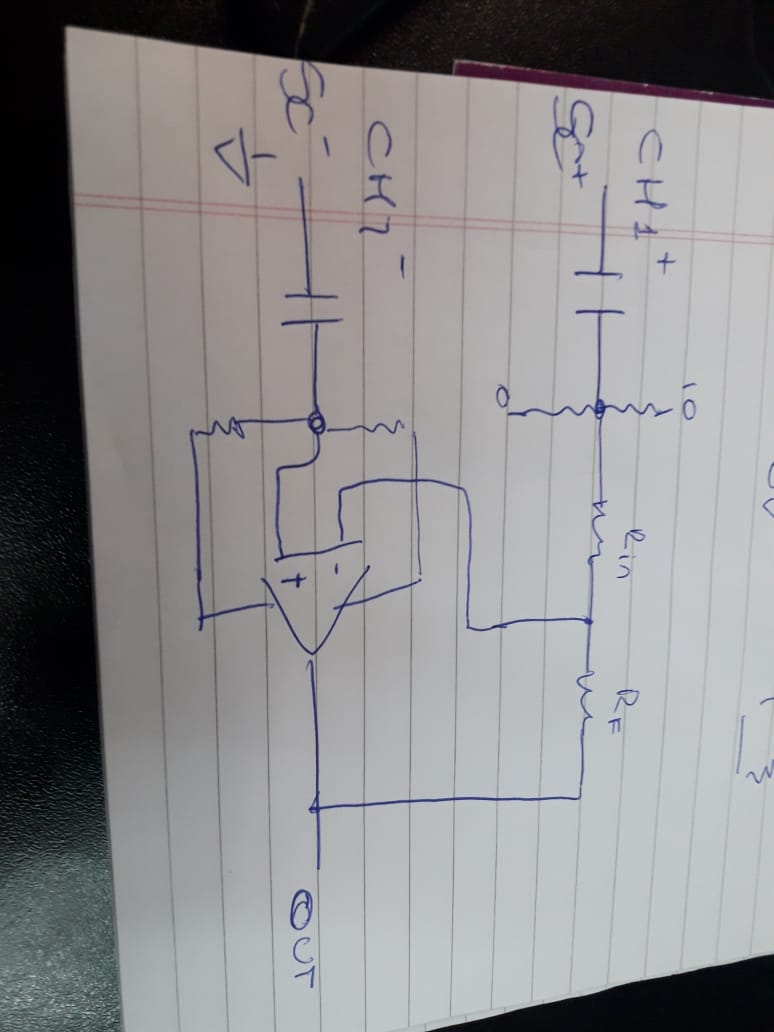
\includegraphics[scale=0.40]{final.jpeg}
     \caption{Al circuito final que usamos le agregamos este div de tension(despues le ponemos un cap)}
     \label{snr_log_micro}
\end{figure}


La continua molestaba porque al no tener el numero referido al 5 v del opamp le sumo la ganancia del OFFSET!!! POR ESO DABA 10 
PARA ELIMINAR ESTA GANANCIA DEL OFFSET PUSIMOS UN CAPACITOR !!!




Por ultimo, medimos el tiempo de bajada y subida del opamp. Le tuvimos que mandar la señal con el generador para enviarle una cuadrada. Lo hicimos para todas las ganancias que hicimos. Con la compu no se la podemos mandar porque necesitariamos una señal mas rapida. (las cone son las mismas que antes pero donde estaba la placa ahora está el gen.) 


\section{dia 21/05}

\subsection{Notas de clase}
Preguntas para hacerse: Como poner a prueba la hoja de daatos de la placa de adqui ? Como diseñar algun exp para pobrar lo que dice la placa? similitudes y diferencias con la placa de audio 

Esquemas de aduquisión: placas o osci 

Digitalizamos porque la queremos guardar en la compu y lo hacemos con un digiti. El transductor la convierte en señal electrica (la prop fisica)y para ir a la compu necesitamos un sistema que adquiera los datos y que lo adapte. 

En esta tapa media (ACONDICIONAMIENTO) podemos:
-amplificar
-aislar: se puede hacer con un transformador(electricamente los circuitos esta aislado). Optoacoplar: replica la señal por medio de luz pero electricamente esta aislado. 
-Multiplexar: le da un ratito a cada entradita con asignacion de prioridades(tiempo)
- Filtrar (pasabajo altos, etc)
- Linealizar: si el transductor no tiene respuesta lineal, asi pesamos todo de la misma manera (los datos lo podemos despues calibrar en la compu pero de esta forma aprovechamos mas la resolucion del dispositivo)
-


Entradas analógicas - DAQ:CARACT:
-frec de muestreo
-multiplexar 
- Rsolucion numero de bits para representar la señal
- rango
- ruido 

OBS: digitalizar es una aprox ==> tiene un error 
Tipos de ADC: 
-Aproximacion sucesiva: compara bit a bit de la señal desde el mas sig al menos sig. Tiene que hacer mas rapido que la tasa de muestreo. 

-Tension a Frec: El circuito convierte la amplitud de interes a una señal de frec tipo tren de pulsosque dependa de la amplitud 

-integracion: Hay un cap que al poner una tension de entrada fija la corriente de entrada y el cap se carga. Despues lo desacoplo de la entrada y lo pongo a una fuente de corriente y hace que el capacitor se descargue. Y midiendo el tiempo total de carga y descarga y asi conozco la tension de entrada con una formulita. 
- Sigma-Delta: del sumador al comparador (de un solo bit y tiene input de Vref, como un DAC)
El conversor me tira algo a cero.
La etapa delta relaciona la tension de entrada con la cantidad de ceros y uno de las pataditas (segun damian esto lo usamos para la placa de audio). No entendí mucho de esto, basicamente es como un integrador ponele (CONSULTAR)


Setting time:
cuando multiplexamos hay un tiempo de respuesta: elegir el orden, la entrda, que la impedancia de entrada sea menor etc. 

TEOREMA DE MUESTRO:
frecuencia de muestreo tiene que ser dos veces mayor a la frecuencia de la señal 

Aliasing: 
cuando no le pego a la frec ... (porq no respeto Nysq)

Resolucion de conversion :
Diapo

Dithering: 
aumentar la resoluc de la conversion: seobremuestrea y promedia 

OBS: VER DIAPO DE RUIDO 

Trigger: es un metodo de sincronizacion. En operaciones sincronizadas esta determinada por el flanco del clock. 

Señales de reloj: 
El clock solo mira el flanco 
diapos de caract. 

Al tener histeresis la señal de ruido podria no subir ni bajar tan facil 

Diagrama de ojo: superponer señales cuadradas . Podemos medir muchas cosas de las que dijo dispersion de estar arriba y abajo, tiempo de subida y bajadas.Mas cerrado es peor. Da idea de la señal digital con la que trabajo. 

Objetivos de mínima
1. Caracterización del efecto de Aliasing
2. Estudiar las configuraciones DIFF, NRSE y RSE
3. Simultaneidad de las mediciones
4. Tiempo muerto entre bloques
5. Armar una hoja de datos para reportar resultados


Usamos en paquete de NI-DAQmx: es super completo entonces es super dificil. Hacer funciones que permitan la facil utilización de este modulo. Es un paquete que habla con un libreria hecha en C. 
\subsection{empezamos}
Estamos usando la placa Vernier SensorDaq (la que dice grupo 6). Segun damian, no tiene Single ended. 

Para la Caracterización del efecto de Aliasing le enviamos una señal con una frecuencia definida y submuestreamos y sobremuestramos. Para esto enviamos unan señal desde la compu con distintas frecuencias. O estamos viendo de hacerlo con un generador.  
La ssalida de la pc (las dos) ls conectamos al 11 y al 12. Estamos haciendo un diferencial. La tierra de la placa esta con la de la compu. 

Queremos hacer lo siguiente: 
-set Freq de muestreo
-Set Ch
- set trigger
- set buffer?????
- por ultimo que mida 

El maximo de puntos que puede tomar el sensor daq es 1024 y no lo reescribi porque prealocamos el vector.  

vamos a hacer subsampleo: (1vPP)

N = 1000 y rate = 1000

Daq01 gen $\_$ frec 1.0000239kHz  

Daq02 gen $\_$ frec 1kHz

N = 1000 y rate = 500

Daq03 gen $\_$ frec 1kHz 

N = 1000 y rate = 100
Daq04 frec $\_$ gen 1Khz


Para unidades en latex ==> SI units 

N = 1000 y rate = 1000
Daq05 FEC 10 MhZ

N = 1000 y rate = 40000
Daq06 FEC 10 MhZ

N = 100 y rate = 2000
Daq07 FEC 1khZ

N = 1000 y rate = 2000
Daq08 FEC 1khZ

N = 1000 y rate = 2100
Daq09 FEC 1khZ

N = 1000 y rate = 2600
Daq10 FEC 1khZ

N = 1000 y rate = 3000
Daq11 FEC 1khZ

N = 1000 y rate = 10000
Daq12 FEC 1khZ

N = 100 y rate = 10000
Daq13 FEC 1khZ

N = 100 y rate = 20000
Daq14 FEC 1khZ

Ya hicimos el paso 1. 

\section{Dia 28/05}
Seguimos con las mediciones del otro dia. 

\begin{figure}
    \centering
    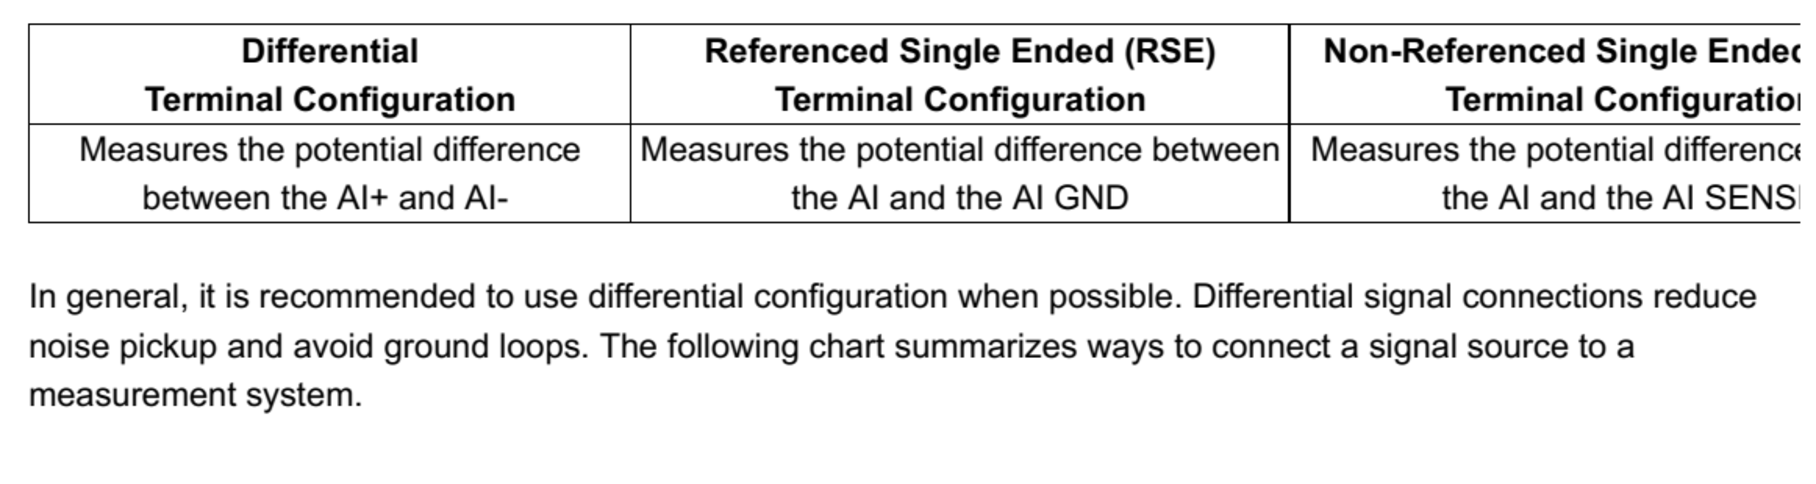
\includegraphics[scale=0.4]{imagenes/SNRE1.pdf}
    \caption{de NI}
    \label{fig:snre1}
\end{figure}

\begin{figure}
    \centering
    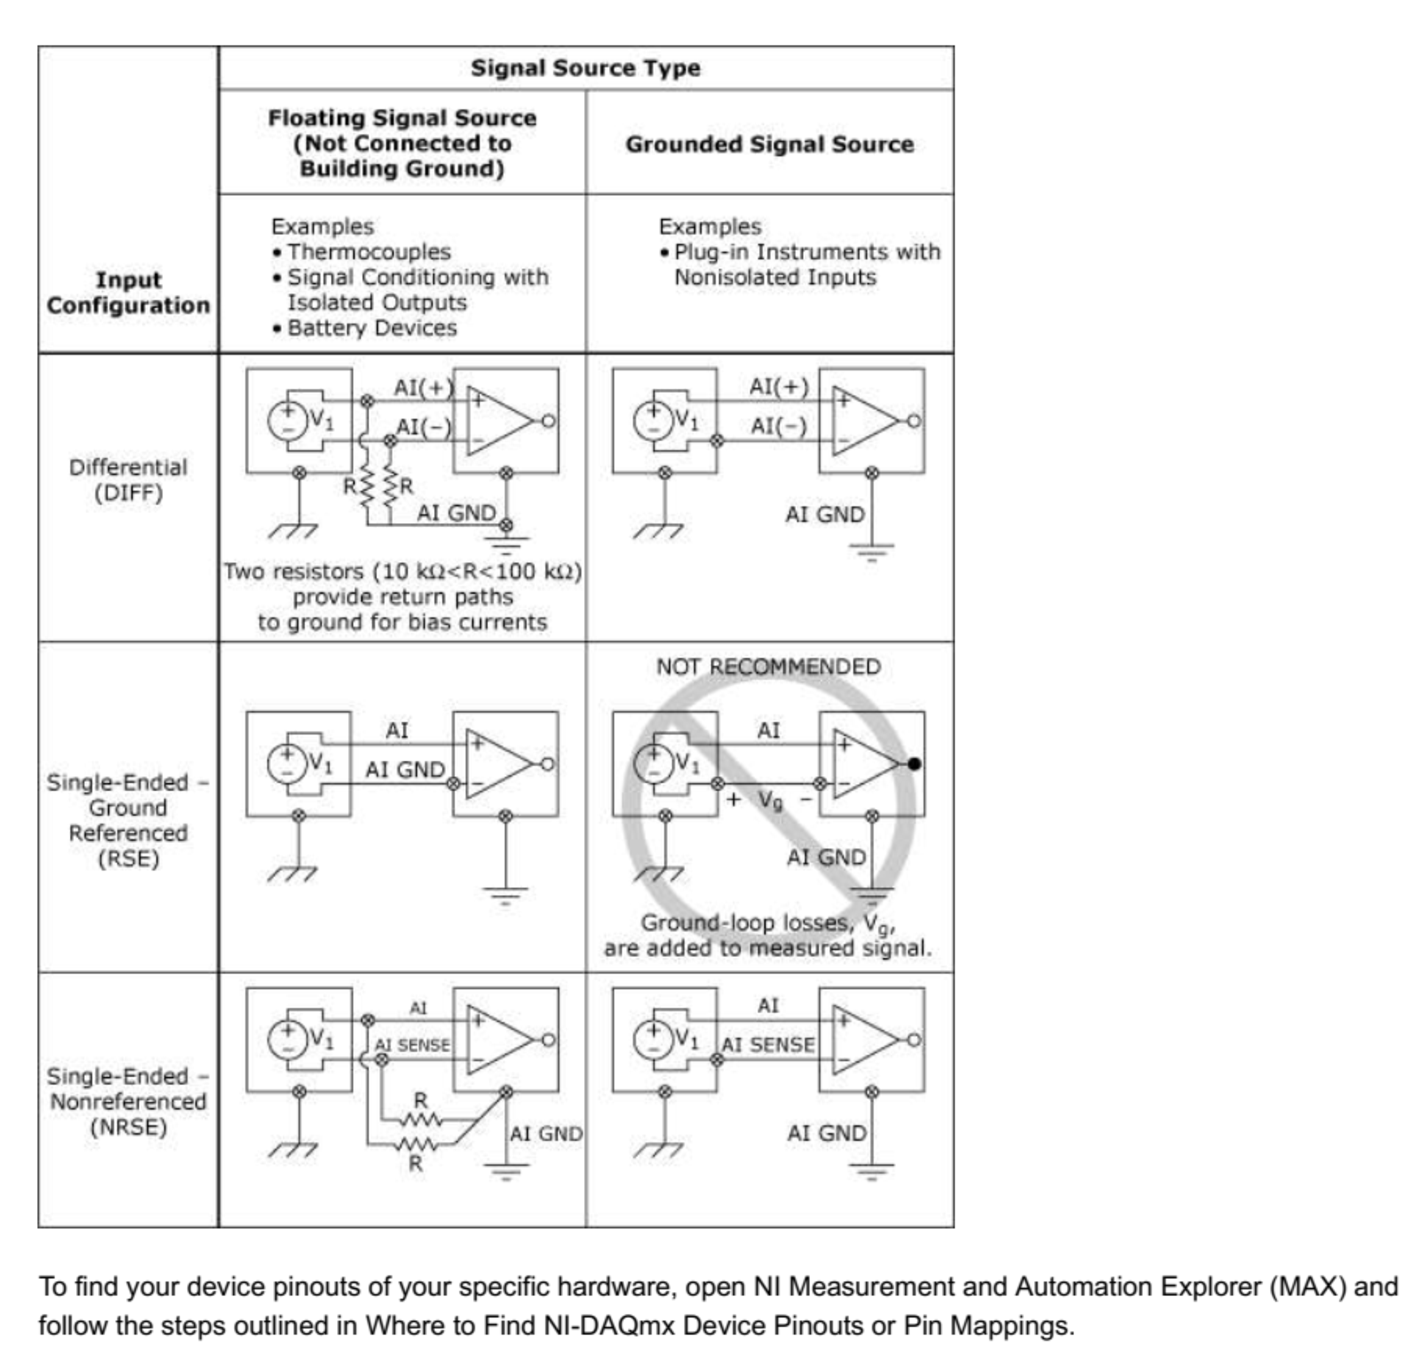
\includegraphics[scale=0.6]{imagenes/SNRE2.pdf}
    \caption{de NI}
    \label{fig:snre2}
\end{figure}

\subsection{RSE y NRSE}

Estamos probando el RSE de la derecha de la fig \ref{fig:snre2}. hicimos la configuracion que funciona MAL osea el + del osci al 12 y el tierra al 10. (eS La confi prohibida). El problema es que el gen esta a tierra NO flotante. 

Diferecial tengo la mitad de canales
en ai sense termina poniendo multiples canales referenciados al mismo punto. 

\begin{enumerate}
    \item daq dia2 1, dejamos suelta la tierra del GF y la tierra del DAQ.
    \item  daq dia 2 2, conectamos el GND del GF y del DAQ juntas en modo RSE (configuración prohibida), así estamos haciendo un loop de tierra. No debería funcionar correctamente.

\end{enumerate}{}

Ambas señales funcionan bien, el problema creemos que proviene que no tenemos un instrumento que esté metiendo ruido en la linea donde está conectado el GF (tal vez un motor?). 

La placa que estamos utilizando (Vernier) no posee modo NRSE, por lo cual no podemos mirar ese caso.

Para configurar el canal en modo RSE y medirlos simultáneamente:
nidaqmx.constants.TerminalConfiguration.RSE (Python attribute, in nidaqmx.constants)
y hay que poner AnalogMultiChannelReader


\begin{enumerate}
    \item daq dia 2 3, N = 1000, rate = 10000, entrada GF, f = 1 kHz, Vpp = 1V. Fila 2 ch 12, Fila 1 ch 11.
    \item daq dia 2 4, N = 1000, rate = 10000, entrada GF, pulso de 10 us y periodo de 1 ms. Fila 2 ch 12, Fila 1 ch 11.
    \item daq dia 2 4, N = 1000, rate = 10000, entrada GF, pulso de 10 us y periodo de 1 ms. Fila 2 ch 12, Fila 1 ch 11.
    \item daq dia 2 5, N = 1000, rate = 10000, entrada GF, pulso de 30 us y periodo de 1 ms. Fila 2 ch 12, Fila 1 ch 11.
    \item daq dia 2 6, N = 1000, rate = 10000, entrada GF, pulso de 500 us y periodo de 1 ms. Fila 2 ch 12, Fila 1 ch 11.
    \item daq dia 2 7, N = 1000, rate = 10000, entrada GF, pulso de 50 us y periodo de 1 ms. Fila 2 ch 12, Fila 1 ch 11. RARA
    \item daq dia 2 8, N = 1000, rate = 10000, entrada GF, pulso de 10 us y periodo de 1 ms. Fila 2 ch 12, Fila 1 ch 11. 
    \item daq dia 2 9, N = 1000, rate = 10000, entrada GF, triangular de Vpp = 1 , f = 1 kHz. Fila 2 ch 12, Fila 1 ch 11.
    \item daq dia 2 10, N = 1000, rate = 10000, entrada GF, pulso de 10 us y periodo de 1 ms. Fila 2 ch 12, Fila 1 ch 11. 
\end{enumerate}{}

Midiendo el GF con el OSC el timempo de crecimiento de la cuadrada que estamos mandando es de 25 ns. Resta determinar a cuál le creemos, al OSC o al GF.

Tiempo usado = Tiempo =np.linspace(0,N*(1/rate),N)


\section{notas de clase }
la idea es poder comunicarnos con los instrumentos con arduinos. 

Tiene un microcontrolador que tiene una mejor programacion que un micro perse. 

Se usa para sensores, robotica sencilla etc. 

Arduino UNO: 
el programa puede pesar 31kB

Se programa en C o casi C

void setup se ejecuta una unica vez (por ejemplo decir que el pin 13 sea OUTPUT)

void loop se ejecuta todo el tiempo


PWM tren de pulsos en la salida con un dutty cicle controlable (xp no tiene un conversor digital). Importa q la frec del pwm sea mas rapida que la que le sigue. 



Objetivo:: programar en arduino y que comunique con python. Y la ventaja es construir cosas indep de la compu. 


En lantz: permite crear clases en arduino. 
boolfeat para booleanos
La comunicacion viene dada gratis pero lo que haga el arduino lo escribimos nosotros 

INO: crea la carpeta con varias cosas. El archivo ppal se llama igual que la carpeta

\subsection{empezaoms con arduino }




\subsection{Sobre el final de la mat}
Pract esp de un dia un dia y medio. Ver algo que tenga que ser sensado con una respuesta de forma activa en el control de una variable físca. 





























































\end{document}
